\section{解析函数}

\subsection{可微性考点}

\begin{itemize}
	\item 判定可微
	\item 判定不可微
	\item C-R 方程
	\item $f$ 在 $z_0$ 解析 $\Rightarrow$ $f$ 在 $z_0$ 可微
	\item $f$ 在 $z_0$ 解析 $\not\Leftarrow$ $f$ 在 $z_0$ 可微
	\begin{itemize}
		\item 存在可微但不解析的点
		\item 解析是一个局部的概念,指的是在 $z_0$ 附近都可微
		\item 可微是一个点态的概念
	\end{itemize}
	\item 极坐标形式的 C-R 方程
	\item 若 $f\in H$ 则 $\overline{\partial}f=0$.
	\item 洛必达法则
\end{itemize}

\begin{exercise}[在 $z_0$ 可微但不解析]
\begin{figure}[H]
\centering
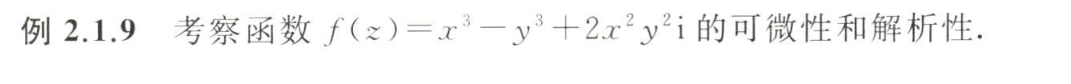
\includegraphics[width=\textwidth]{4-解析函数-20250320.png}
% \caption{}
\label{}
\end{figure}
\end{exercise}
\begin{figure}[H]
\centering
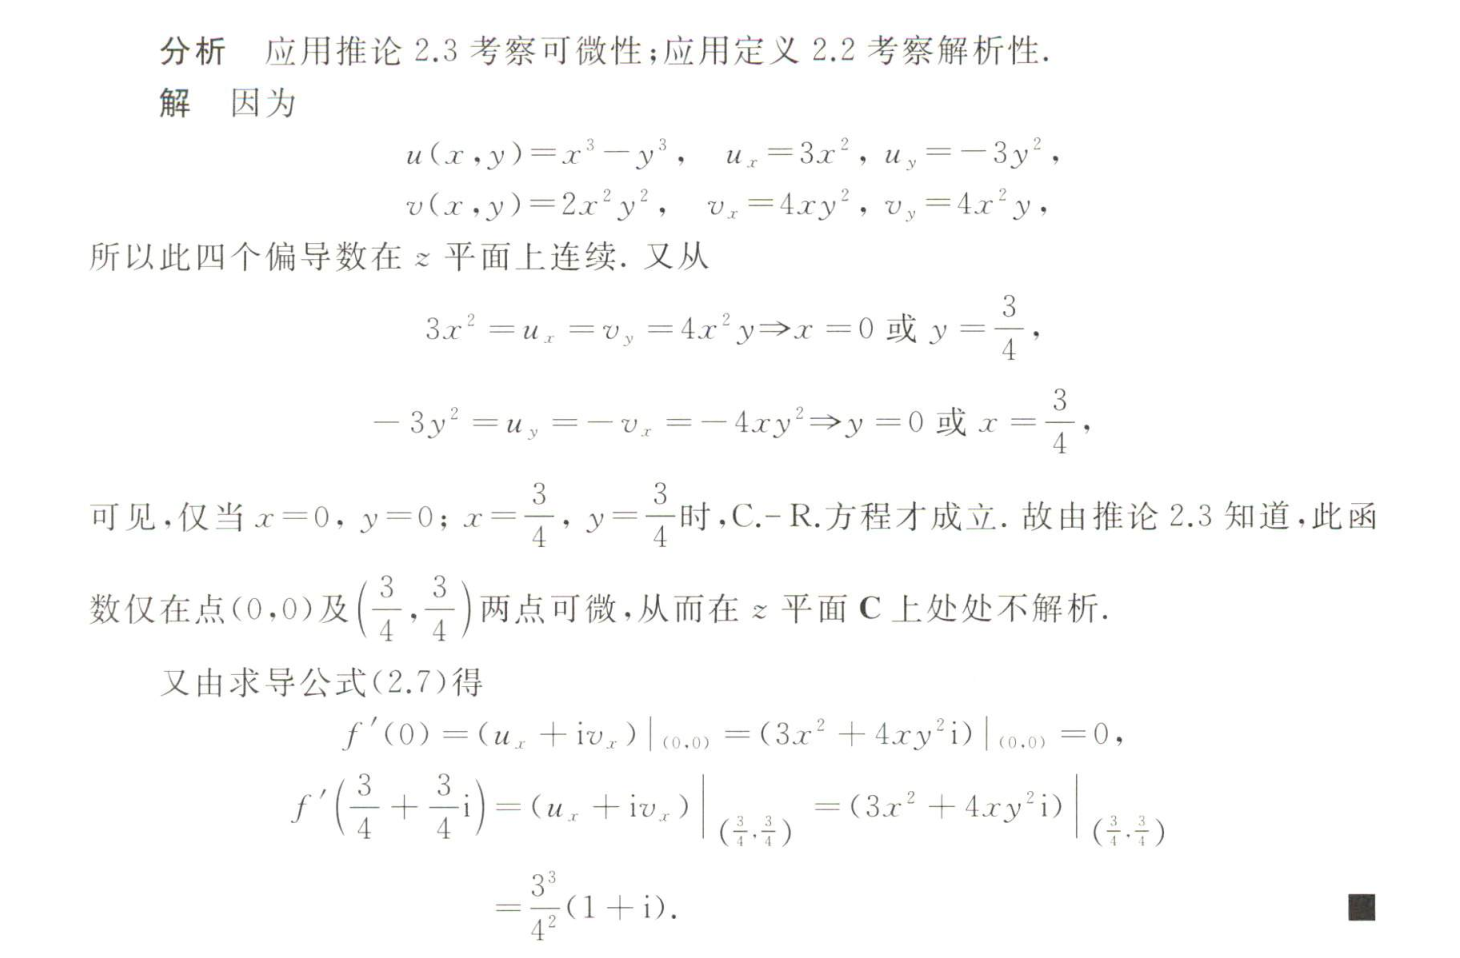
\includegraphics[width=\textwidth]{5-解析函数-20250320.png}
% \caption{}
\label{}
\end{figure}

\begin{remark}
\begin{figure}[H]
\centering
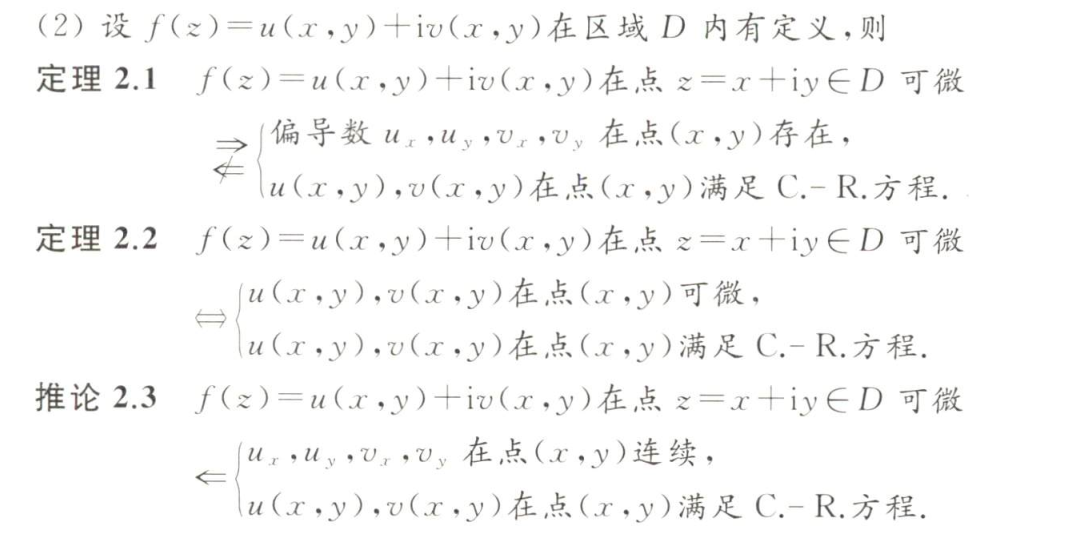
\includegraphics[width=\textwidth]{解析函数-20250320.png}
% \caption{}
\label{}
\end{figure}
\begin{figure}[H]
\centering
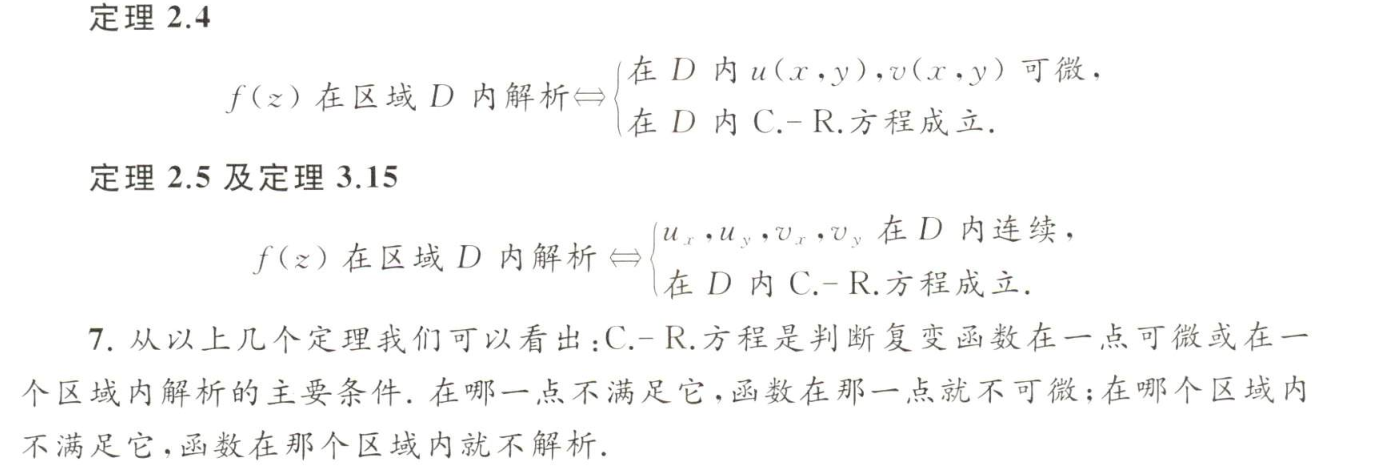
\includegraphics[width=\textwidth]{1-解析函数-20250320.png}
% \caption{}
\label{}
\end{figure}
\end{remark}
\begin{figure}[H]
\centering
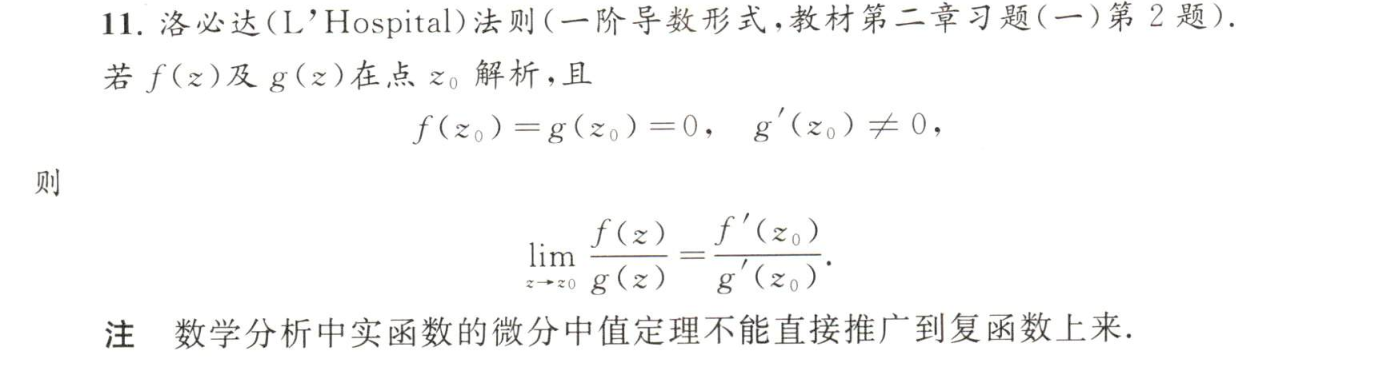
\includegraphics[width=\textwidth]{3-解析函数-20250320.png}
% \caption{}
\label{}
\end{figure}

\subsection{初等解析函数}

考点:

\begin{itemize}
	\item $e^{ z_1 }=e^{ z_2 }\iff z_1=z_2+2k\pi i$. $k\in \mathbb{Z}$.
	\item $\sin z=\frac{1}{2i}(e^{ iz }-e^{ -iz }),\cos z=\frac{1}{2}(e^{ iz }+e^{ -iz })$
	\item 在 $\mathbb{C}$ 不能断言 $\lvert \sin z \rvert\leq1,\lvert \cos z \rvert\leq1$.
	\item 证明 $f(z)$ 的一致连续性和不一致连续性
	\item $\tan z=\frac{\sin z}{\cos z},\cot z=\frac{\cos z}{\sin z}$.
	\begin{itemize}
		\item $\cos z$ 的零点 $\left ( n+\frac{1}{2} \right)\pi, n\in \mathbb{Z}$ 是 $\tan z$ 在 $\mathbb{C}$ 的全部奇点
		\item $\sin z$ 的零点 $n\pi, n\in \mathbb{Z}$,是 $\cot z$ 在 $\mathbb{C}$ 的全部奇点
	\end{itemize}
	\item $\sinh z=\sin\left( \frac{z}{i} \right),\cosh z=\cos\left( \frac{z}{i} \right)$
\end{itemize}

\begin{exercise}
证明
\[
\lim_{ n \to \infty } \left( 1+\frac{z}{n} \right)^{n}=e^{ z }
\]
\end{exercise}
\begin{proof}
只需证明
\[
\lim_{ n \to \infty } \left\lvert  \left( 1+\frac{z}{n} \right)  \right\rvert ^{n}=e^{ x }
\]
\[
\lim_{ n \to \infty } \arg\left( 1+\frac{z}{n} \right)^{n}=\arg e^{ z }=y
\]
\end{proof}

\begin{exercise}
\begin{figure}[H]
\centering
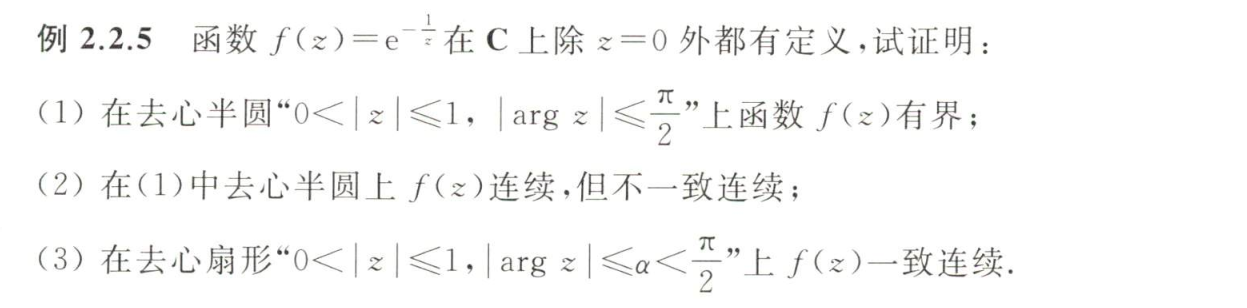
\includegraphics[width=\textwidth]{6-解析函数-20250320.png}
% \caption{}
\label{}
\end{figure}
\end{exercise}
\begin{proof}
\begin{figure}[H]
\centering
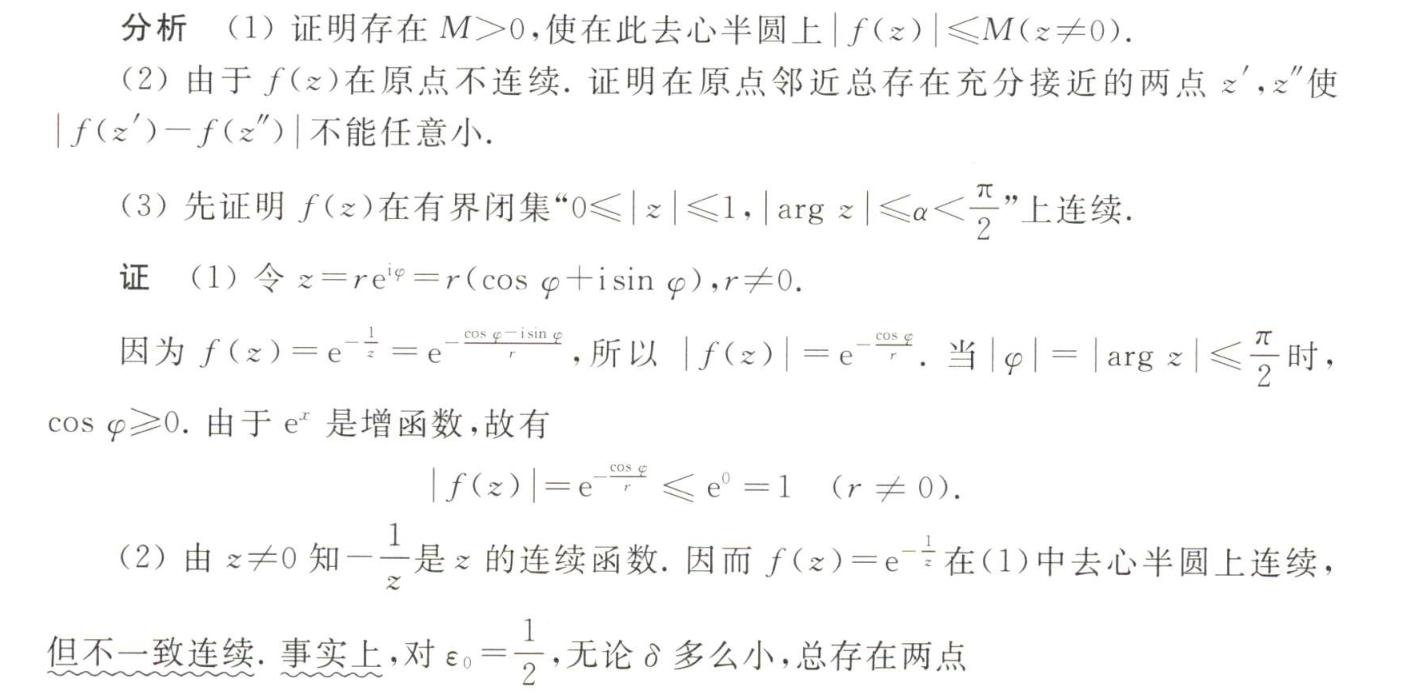
\includegraphics[width=\textwidth]{7-解析函数-20250320.png}
% \caption{}
\label{}
\end{figure}

\begin{figure}[H]
\centering
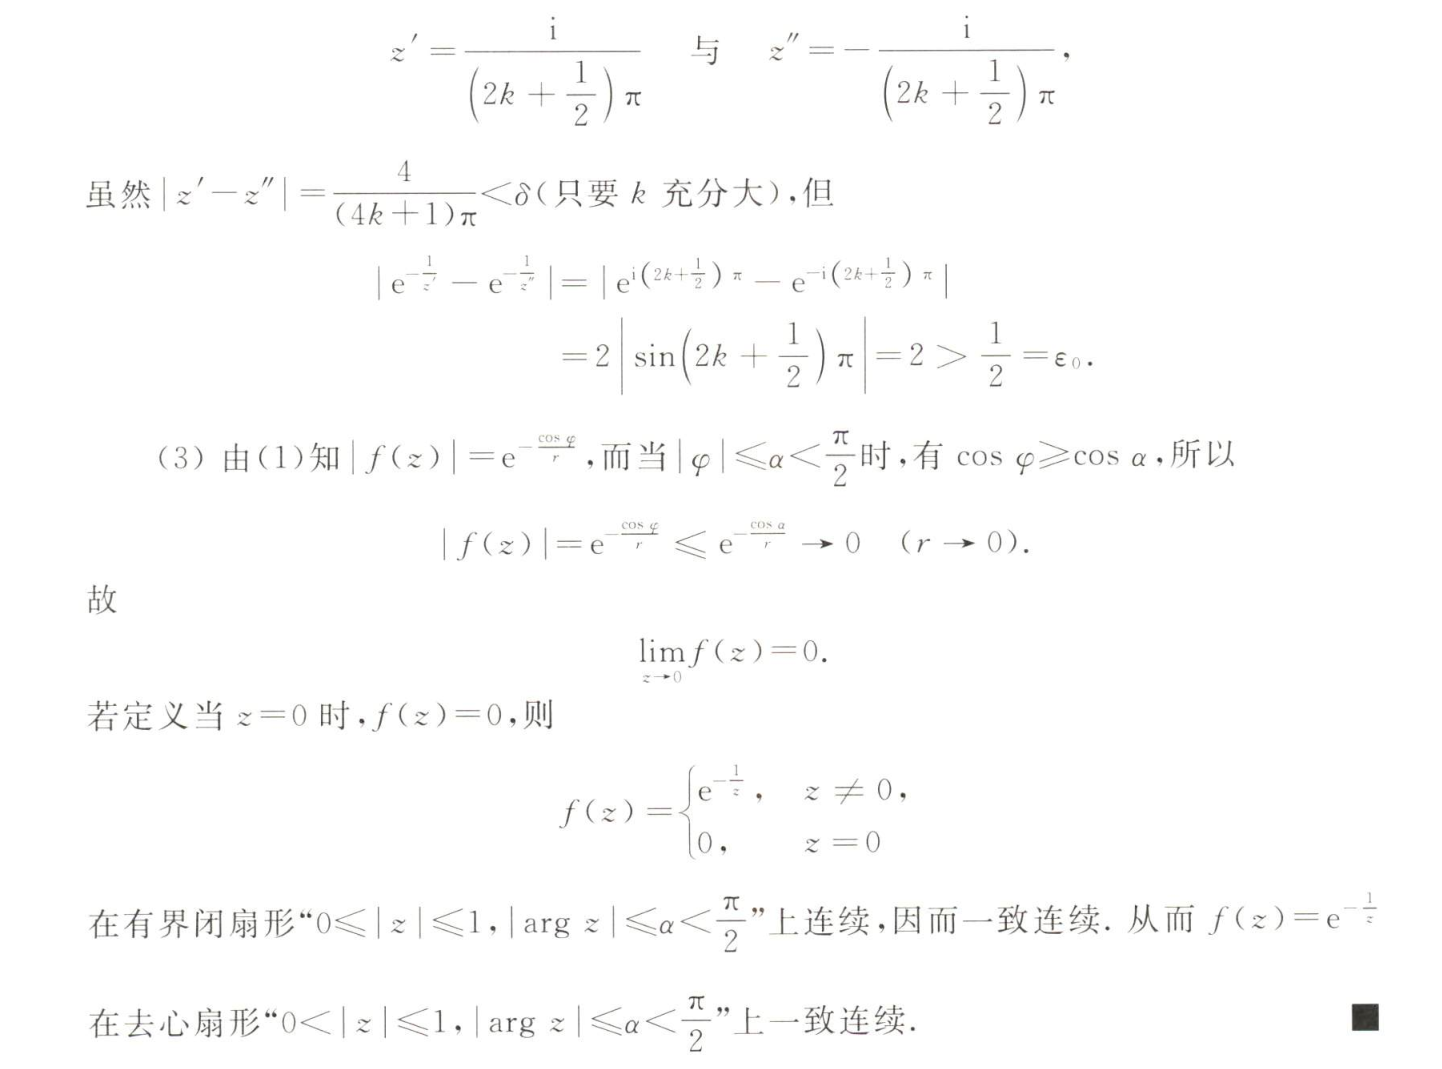
\includegraphics[width=\textwidth]{9-解析函数-20250320.png}
% \caption{}
\label{}
\end{figure}

\end{proof}

\subsection{初等多值函数}

这一节的主要内容是采用限制辐角或割破平面的方法,来分出根式函数和对数函数的单值解析分支。

\begin{figure}[H]
\centering
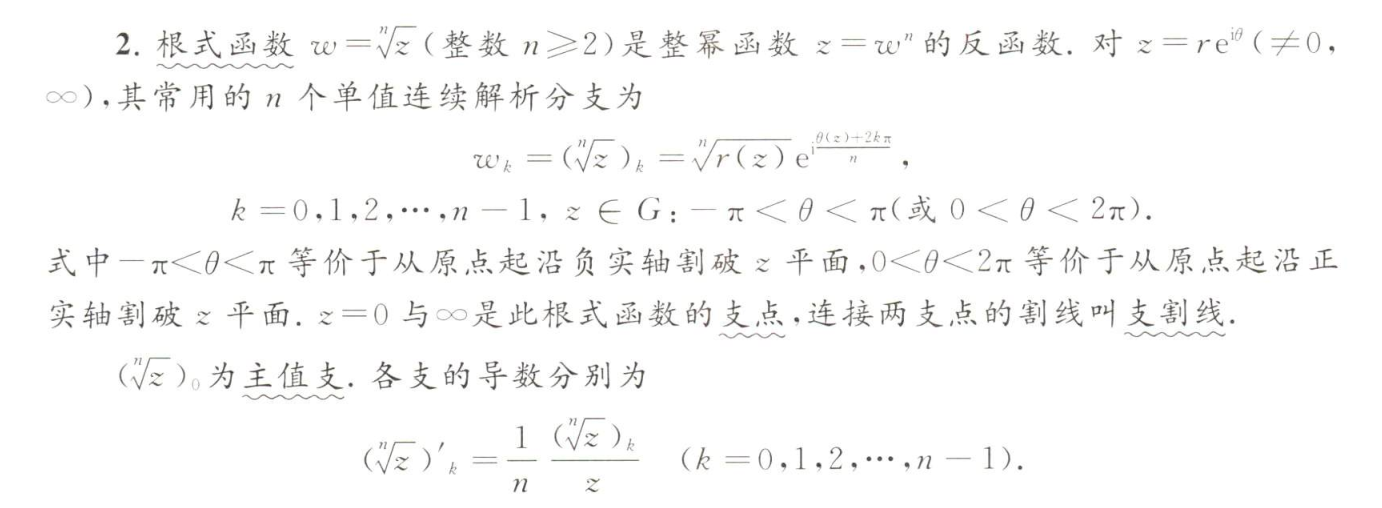
\includegraphics[width=\textwidth]{10-解析函数-20250320.png}
% \caption{}
\label{}
\end{figure}

\begin{exercise}
\begin{figure}[H]
\centering
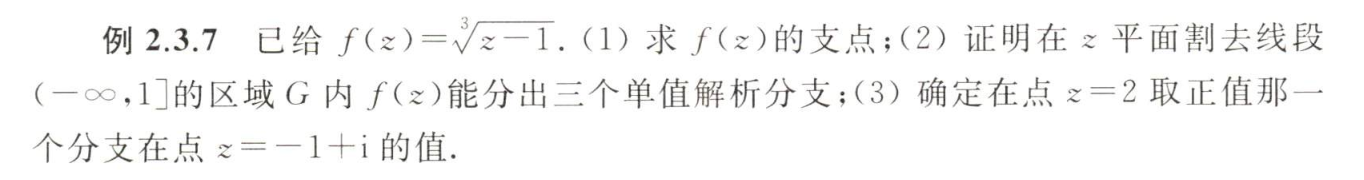
\includegraphics[width=\textwidth]{11-解析函数-20250320.png}
% \caption{}
\label{}
\end{figure}
\end{exercise}
\begin{figure}[H]
\centering
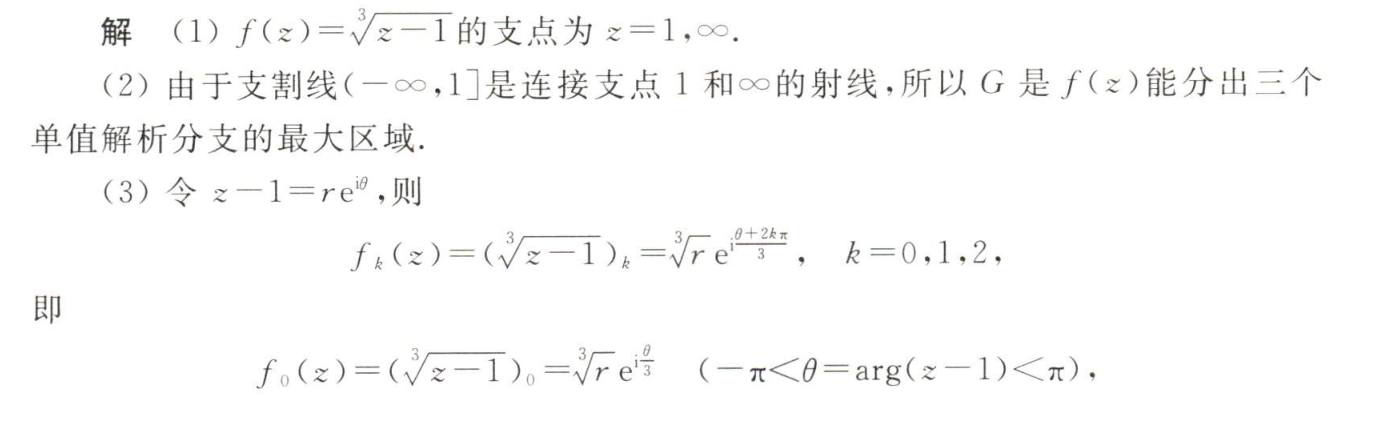
\includegraphics[width=\textwidth]{12-解析函数-20250320.png}
% \caption{}
\label{}
\end{figure}

\begin{figure}[H]
\centering
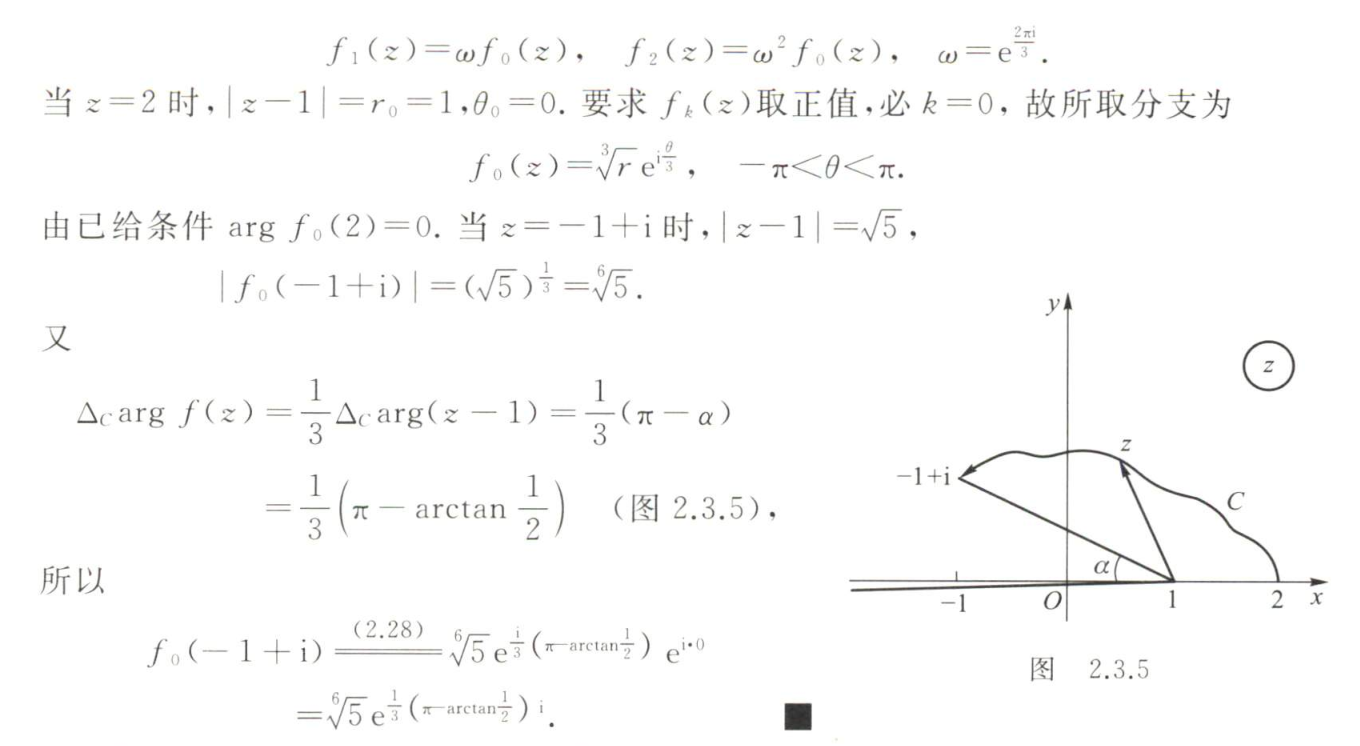
\includegraphics[width=\textwidth]{13-解析函数-20250320.png}
% \caption{}
\label{}
\end{figure}

\begin{figure}[H]
\centering
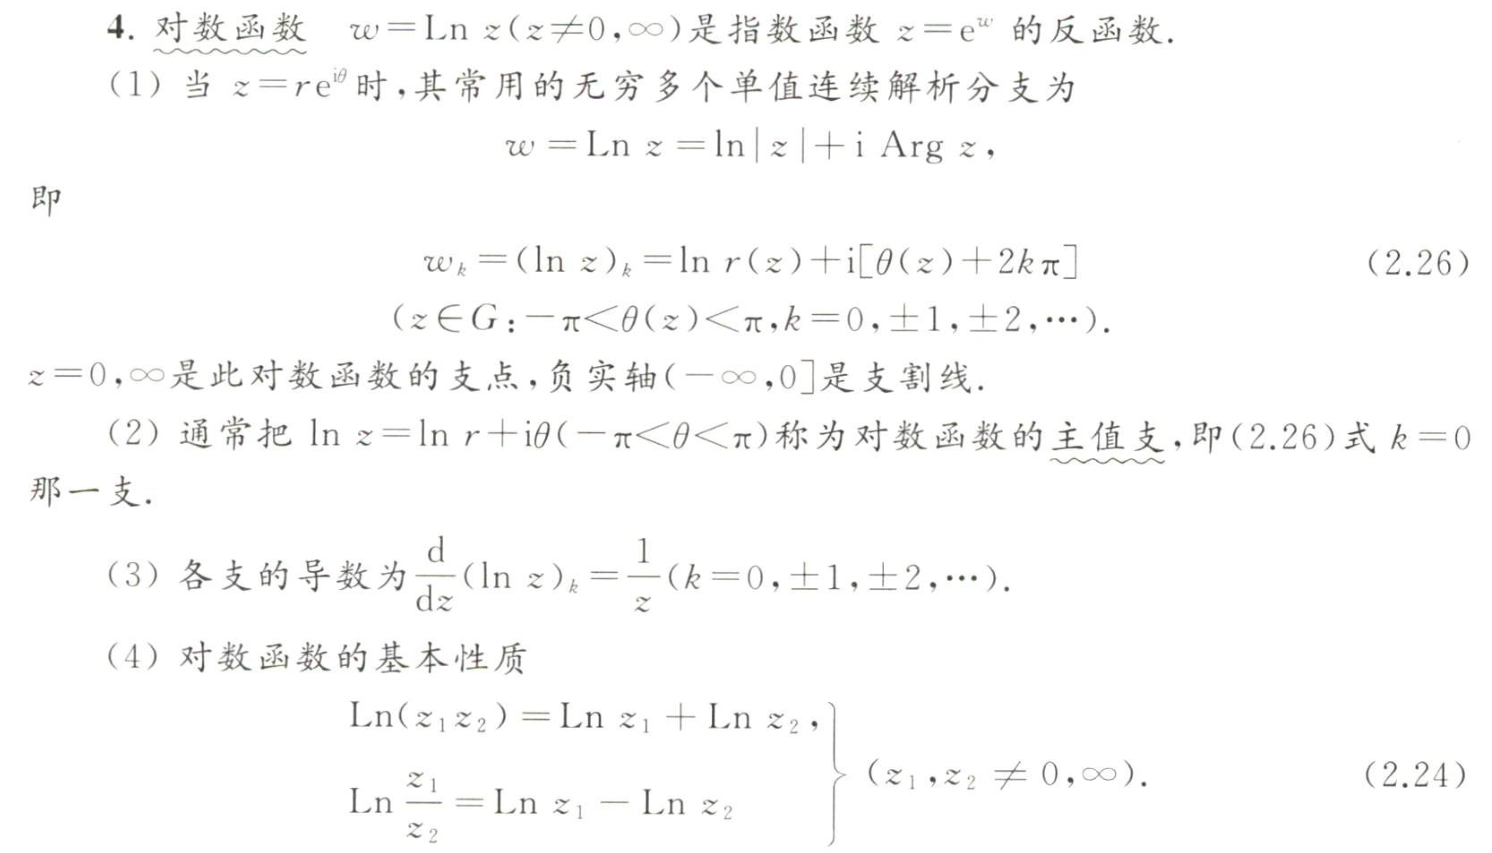
\includegraphics[width=\textwidth]{14-解析函数-20250320.png}
% \caption{}
\label{}
\end{figure}

\begin{figure}[H]
\centering
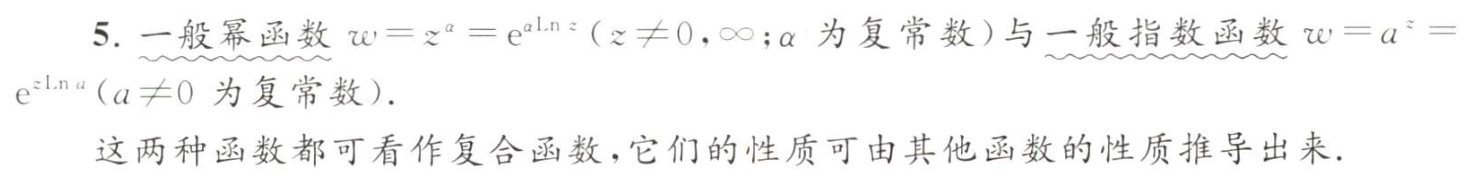
\includegraphics[width=\textwidth]{15-解析函数-20250320.png}
% \caption{}
\label{}
\end{figure}

\subsection{具有多个有限支点的多值函数}

\begin{figure}[H]
\centering
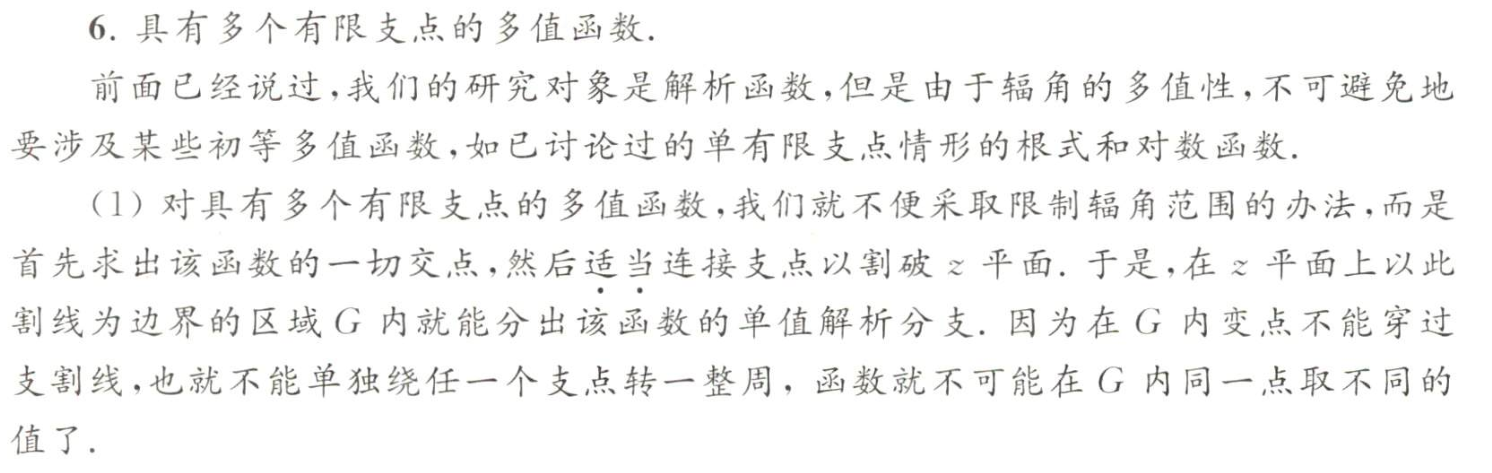
\includegraphics[width=\textwidth]{17-解析函数-20250320.png}
% \caption{}
\label{}
\end{figure}

\begin{figure}[H]
\centering
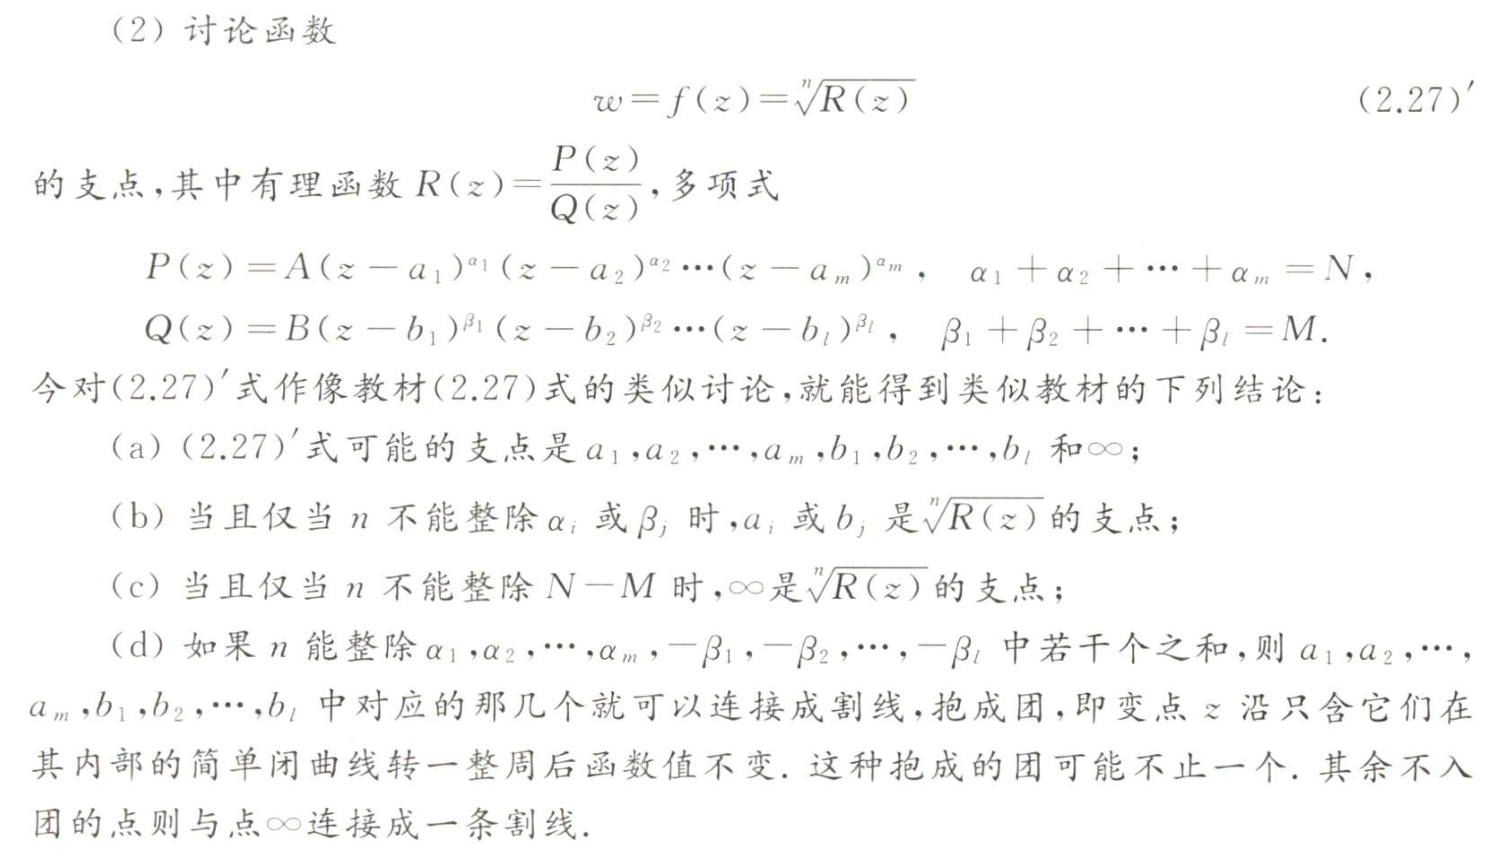
\includegraphics[width=\textwidth]{18-解析函数-20250320.png}
% \caption{}
\label{}
\end{figure}

\begin{figure}[H]
\centering
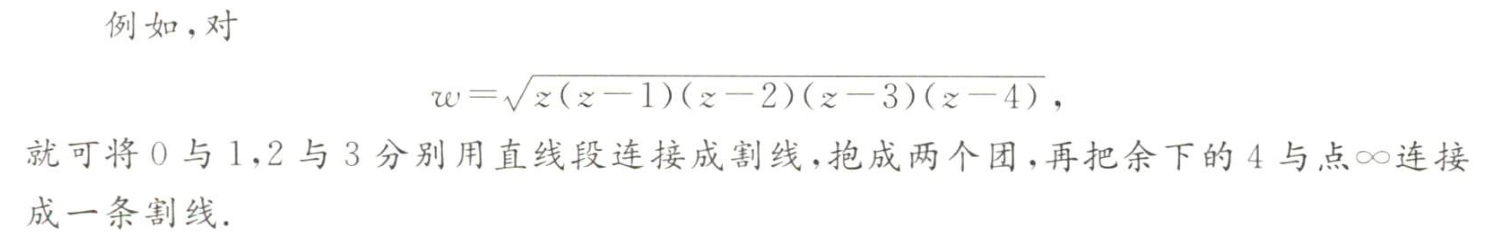
\includegraphics[width=\textwidth]{19-解析函数-20250320.png}
% \caption{}
\label{}
\end{figure}

\begin{figure}[H]
\centering
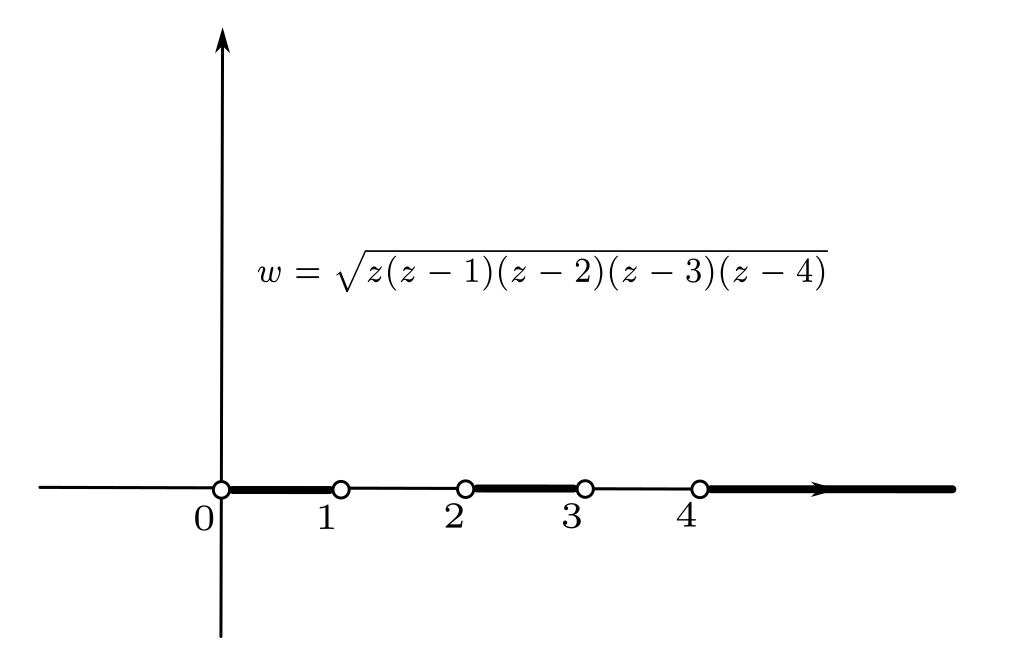
\includegraphics[width=\textwidth]{22-解析函数-20250320.png}
% \caption{}
\label{}
\end{figure}

\begin{figure}[H]
\centering
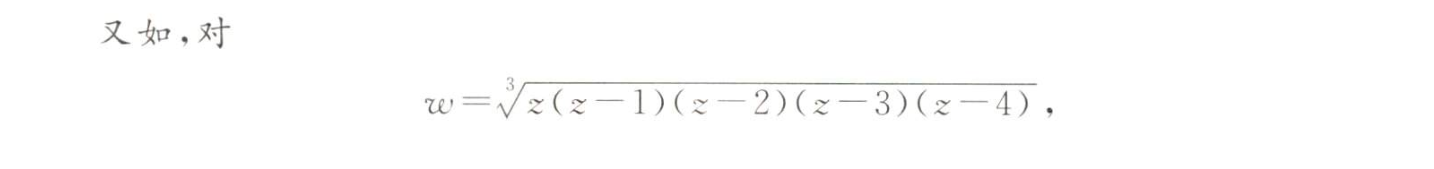
\includegraphics[width=\textwidth]{20-解析函数-20250320.png}
% \caption{}
\label{}
\end{figure}

\begin{figure}[H]
\centering
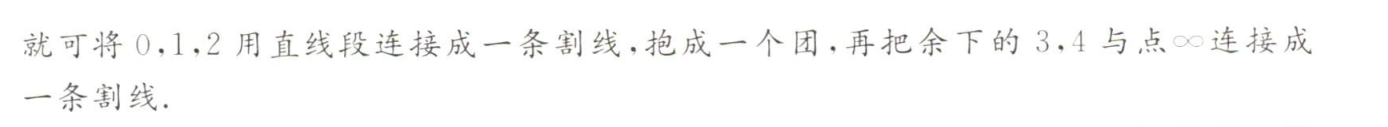
\includegraphics[width=\textwidth]{21-解析函数-20250320.png}
% \caption{}
\label{}
\end{figure}

\begin{figure}[H]
\centering
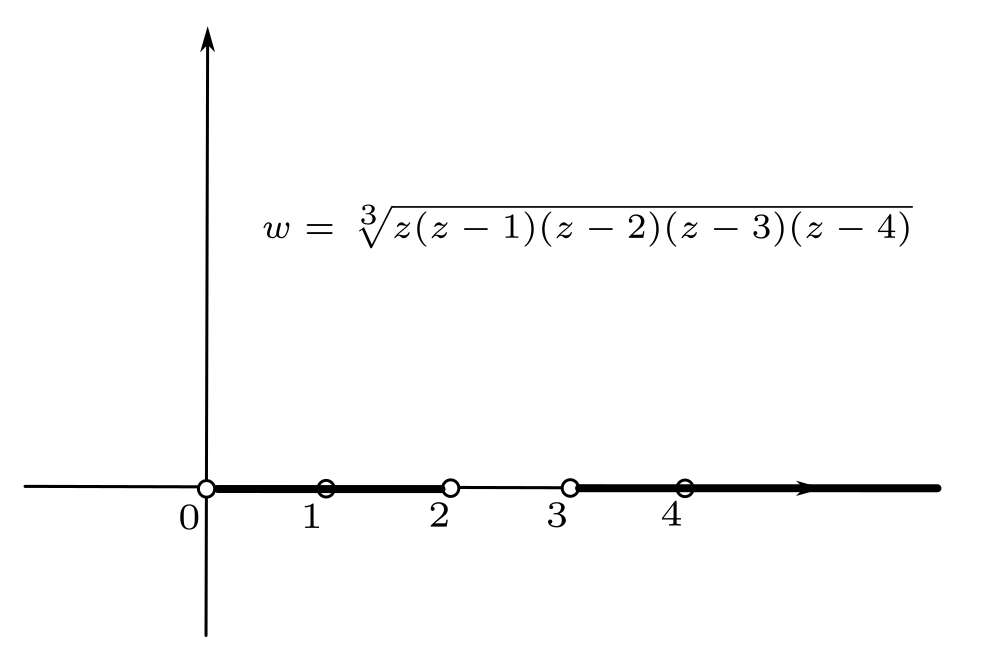
\includegraphics[width=\textwidth]{23-解析函数-20250320.png}
% \caption{}
\label{}
\end{figure}

由已给单值解析分支 $f(z)$ 的初值 $f(z_1)$,计算终值 $f(z_2)$ 的公式为
\[
f(z_2)=\lvert f(z_2) \rvert e^{ i\Delta_{C}\arg f(z) }e^{ i\arg f(z_1) }
\]
其中 $C$ 为连接起点 $z_1$ 和终点 $z_2$ 且不穿过支割线的路线.

当把 $z_2\in G$ 换成 $G$ 的动点 $z$ 时,得到的
\[
f(z)=\lvert f(z) \rvert e^{ i\Delta_{C}\arg f(z) }e^{ i\arg f(z_1) }
\]
也是此单值解析分支的解析表达式.

\begin{exercise}
\begin{figure}[H]
\centering
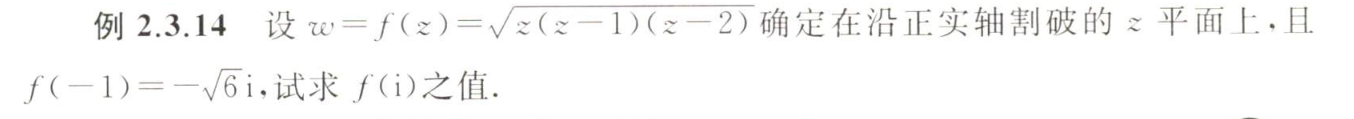
\includegraphics[width=\textwidth]{24-解析函数-20250320.png}
% \caption{}
\label{}
\end{figure}
\end{exercise}
\begin{figure}[H]
\centering
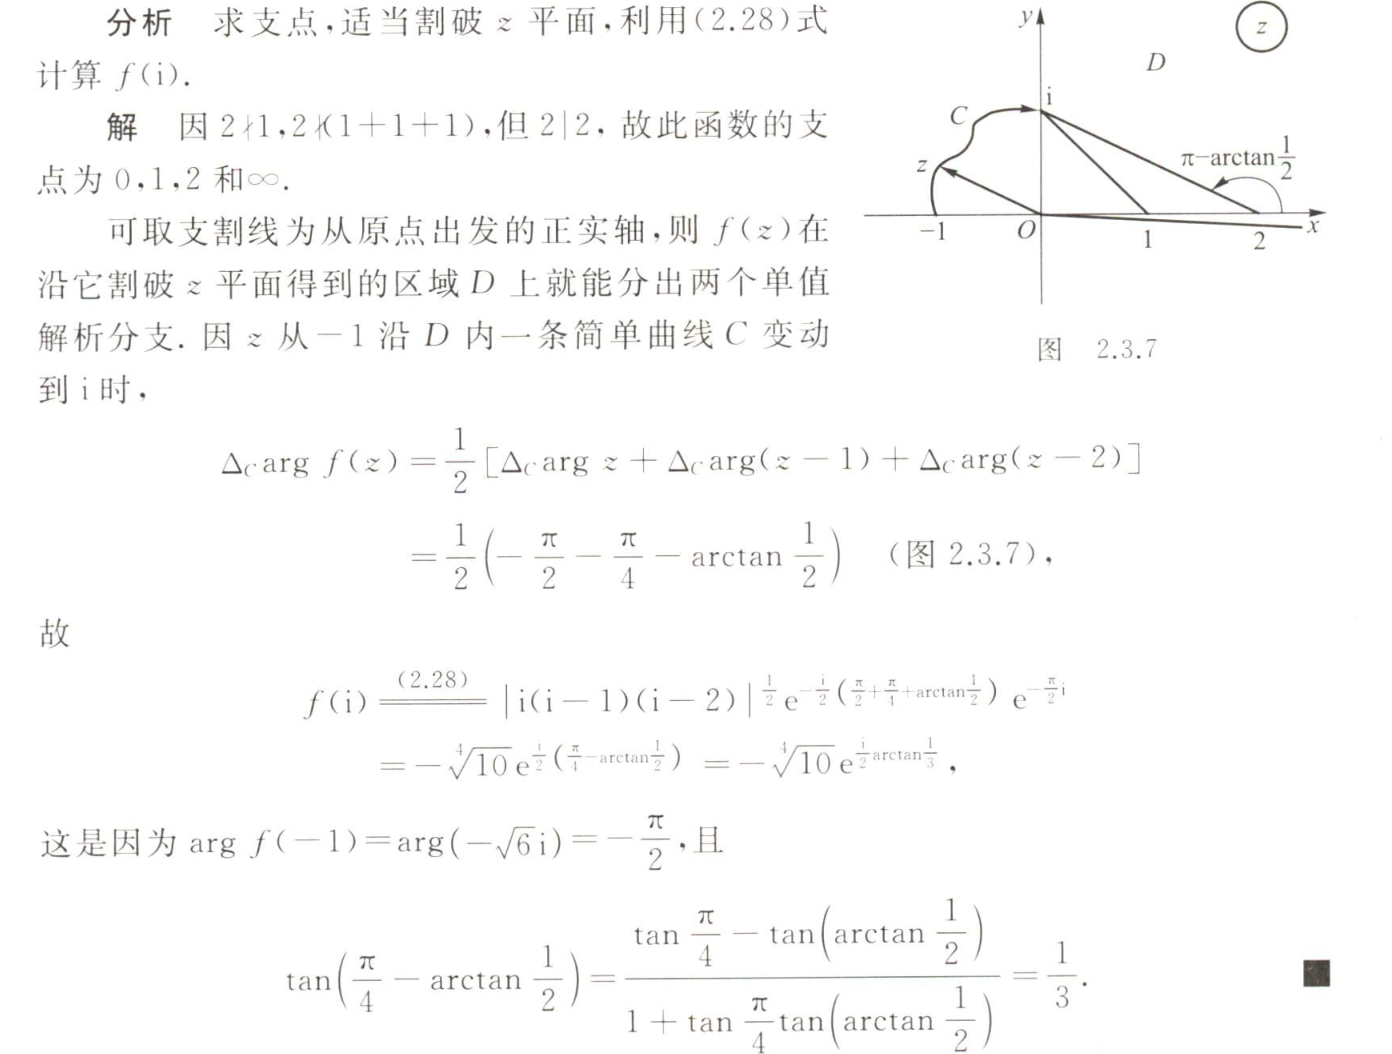
\includegraphics[width=\textwidth]{25-解析函数-20250320.png}
% \caption{}
\label{}
\end{figure}

\begin{exercise}
\begin{figure}[H]
\centering
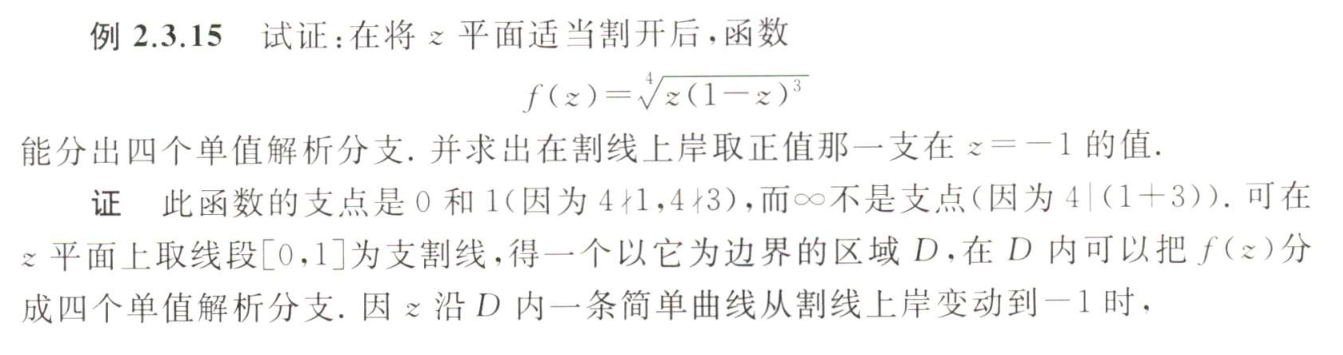
\includegraphics[width=\textwidth]{26-解析函数-20250320.png}
% \caption{}
\label{}
\end{figure}
\end{exercise}
\begin{figure}[H]
\centering
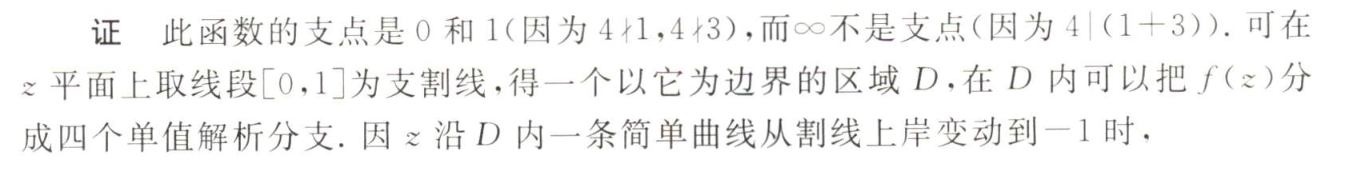
\includegraphics[width=\textwidth]{27-解析函数-20250320.png}
% \caption{}
\label{}
\end{figure}

\begin{figure}[H]
\centering
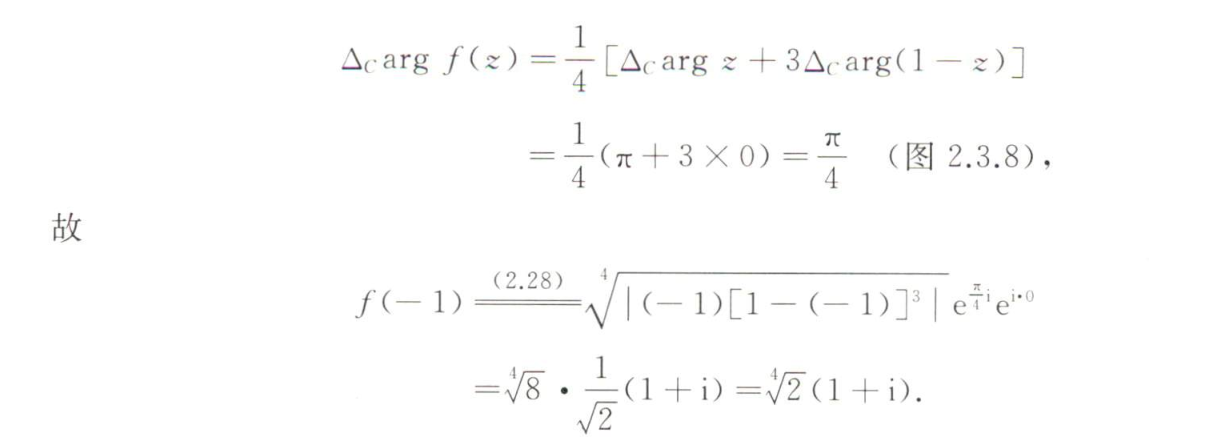
\includegraphics[width=\textwidth]{28-解析函数-20250320.png}
% \caption{}
\label{}
\end{figure}

\begin{figure}[H]
\centering
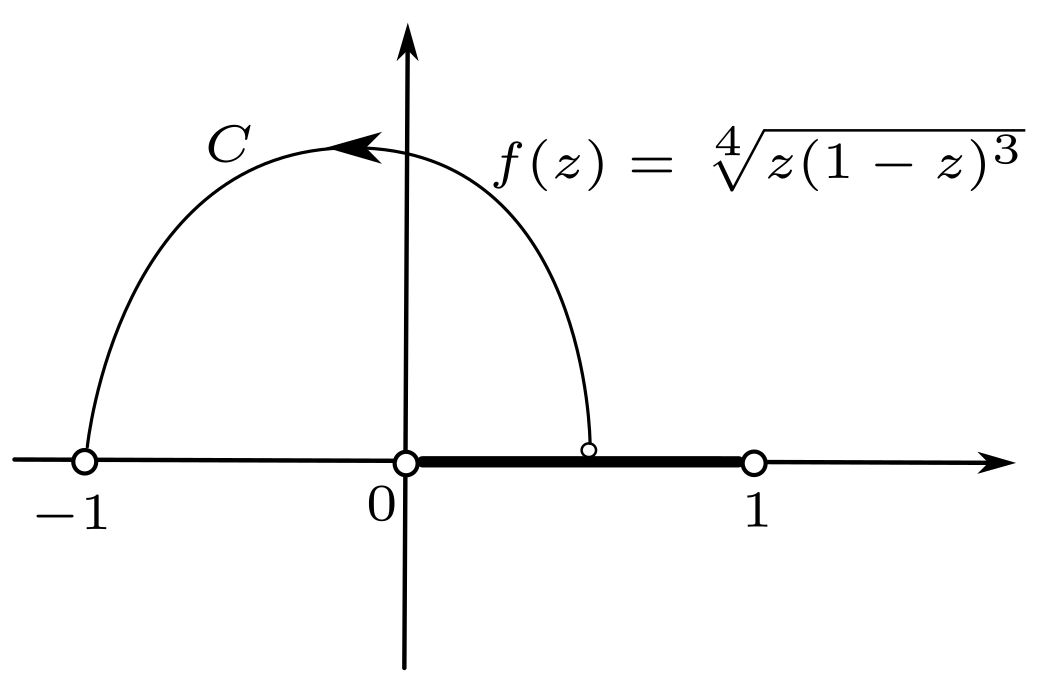
\includegraphics[width=\textwidth]{29-解析函数-20250320.png}
% \caption{}
\label{}
\end{figure}

\begin{exercise}
\begin{figure}[H]
\centering
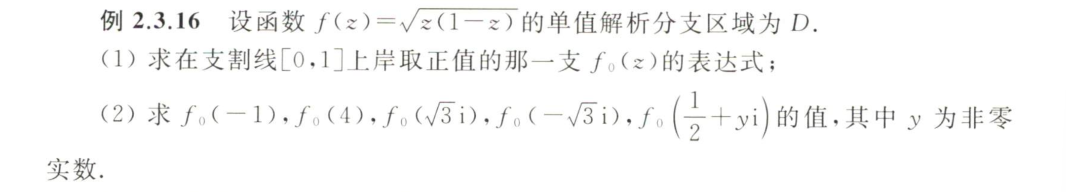
\includegraphics[width=\textwidth]{30-解析函数-20250320.png}
% \caption{}
\label{}
\end{figure}
\end{exercise}
\begin{figure}[H]
\centering
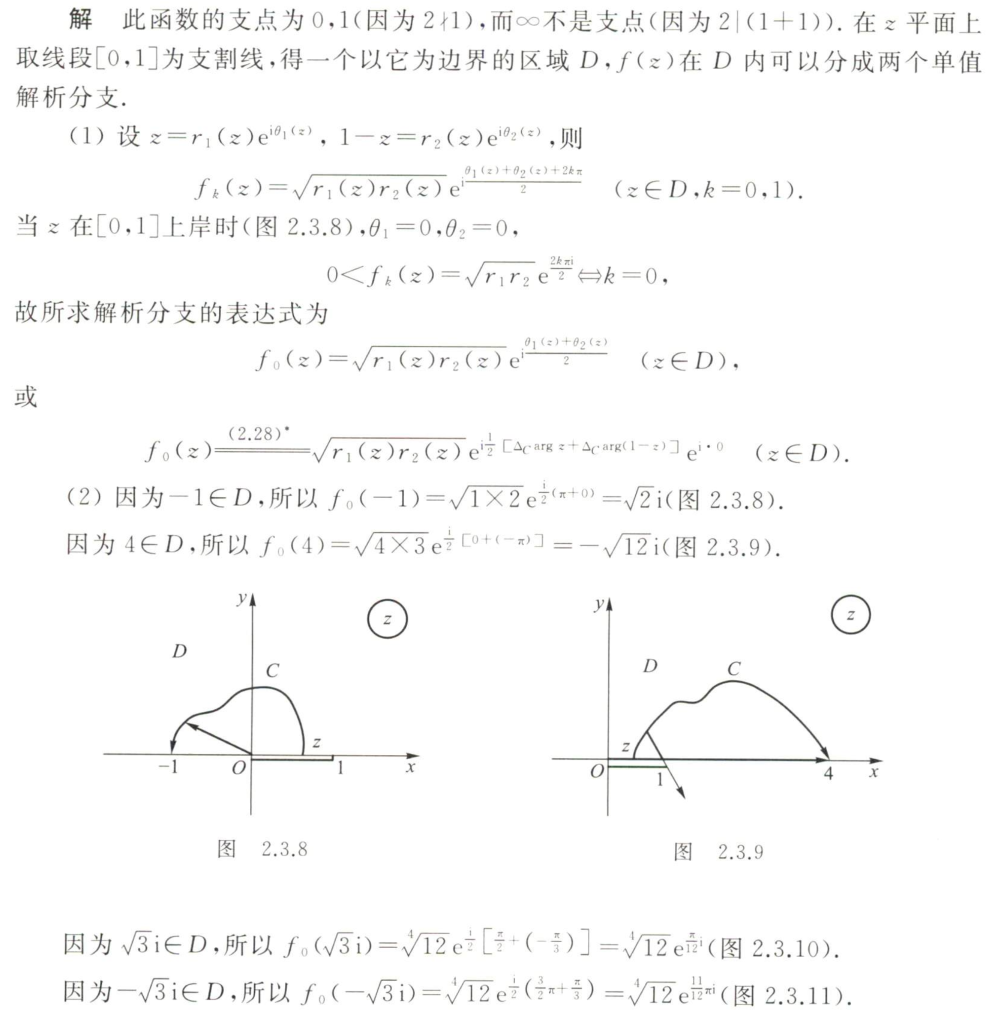
\includegraphics[width=\textwidth]{31-解析函数-20250320.png}
% \caption{}
\label{}
\end{figure}

\begin{figure}[H]
\centering
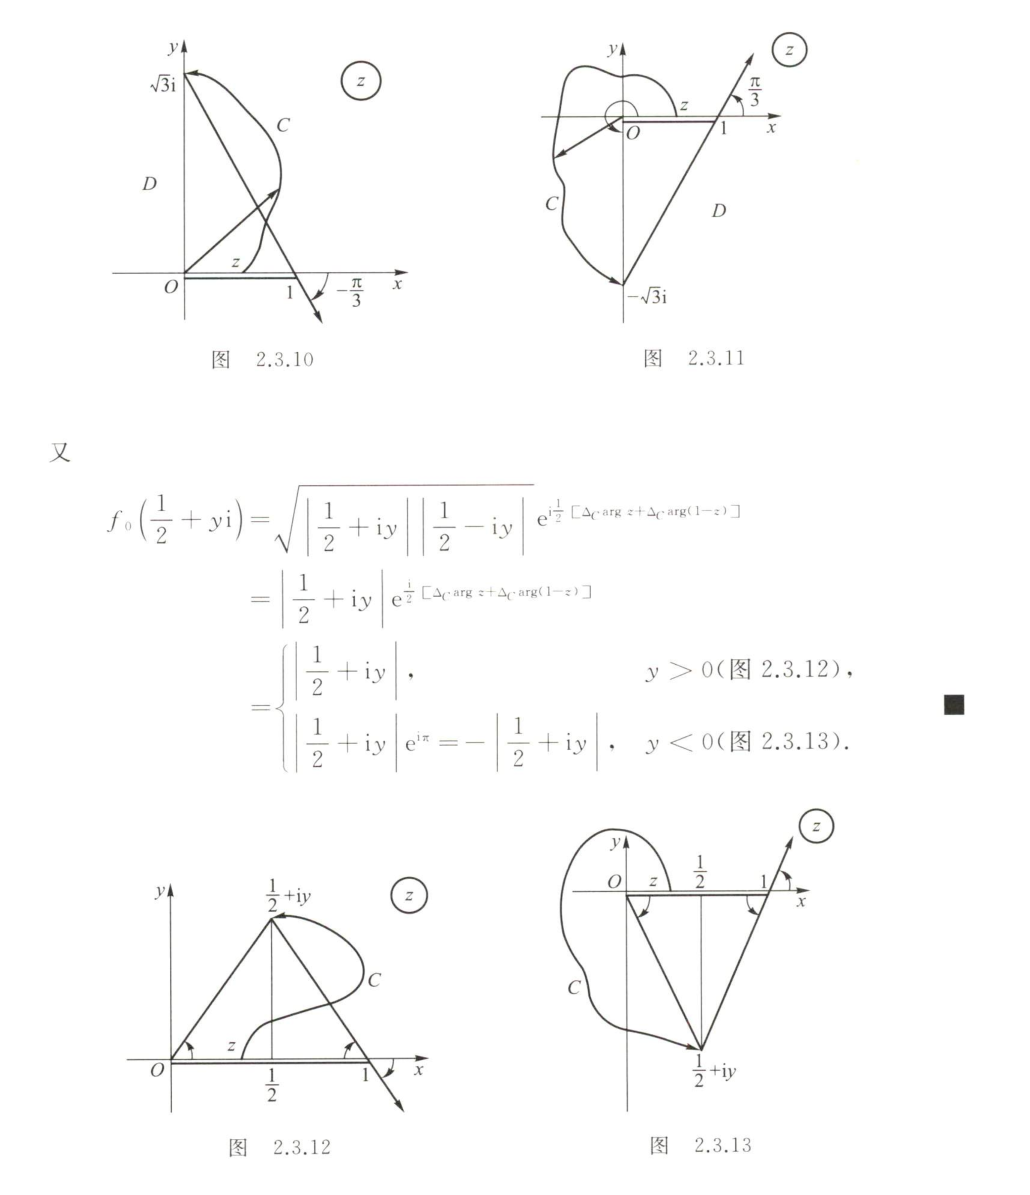
\includegraphics[width=\textwidth]{32-解析函数-20250320.png}
% \caption{}
\label{}
\end{figure}

\begin{exercise}
\begin{figure}[H]
\centering

\includegraphics[width=\textwidth]{33-解析函数-20250320.png}
% \caption{}
\label{}
\end{figure}
\end{exercise}
\begin{figure}[H]
\centering
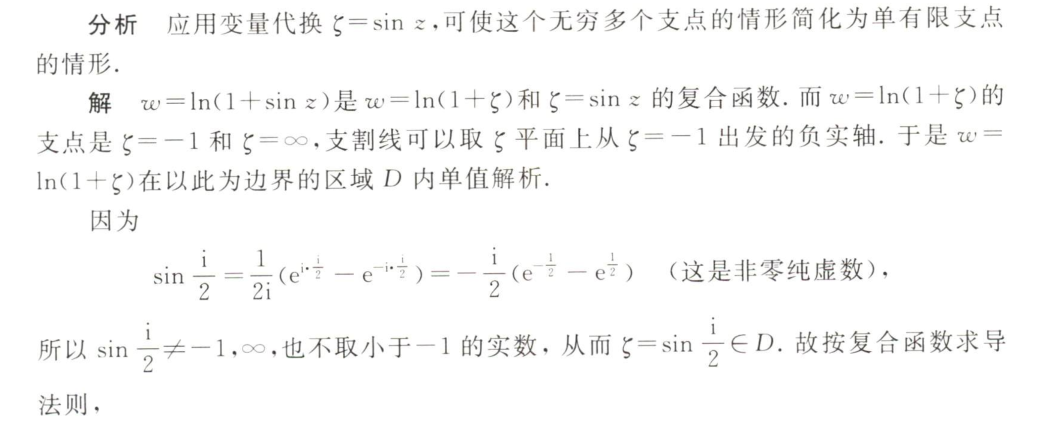
\includegraphics[width=\textwidth]{34-解析函数-20250320.png}
% \caption{}
\label{}
\end{figure}

\begin{figure}[H]
\centering
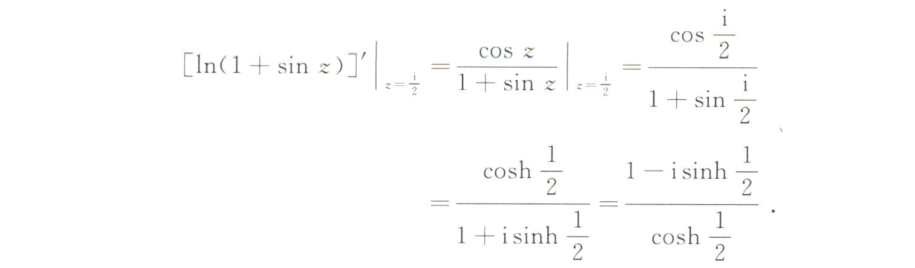
\includegraphics[width=\textwidth]{35-解析函数-20250320.png}
% \caption{}
\label{}
\end{figure}

\subsubsection{反三角函数}

\begin{figure}[H]
\centering
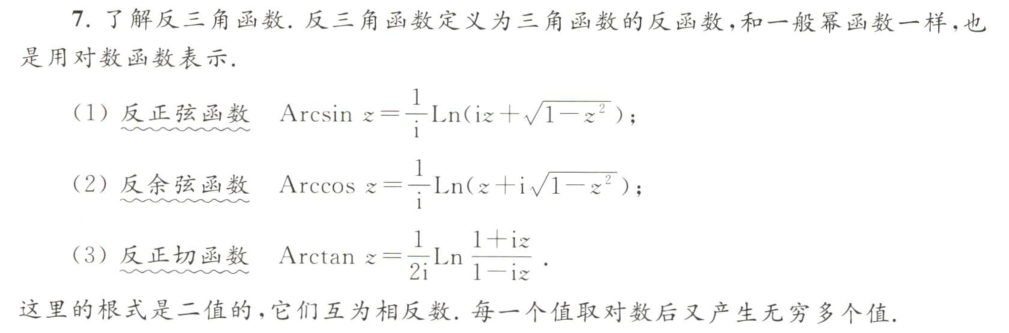
\includegraphics[width=\textwidth]{36-解析函数-20250320.png}
% \caption{}
\label{}
\end{figure}

\begin{note}
所有这些函数分成单值解析分支的方法,与我们前面用过的讨论方法是类似的,也要先讨论它们的支点,然后适当割破平面,只是较复杂些也较困难些。当然也可以像例 2.3.17 和例 2.3.19 一样,把他们视为复合函数来化简处理。
\end{note}
\begin{exercise}
\begin{figure}[H]
\centering
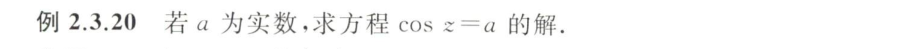
\includegraphics[width=\textwidth]{37-解析函数-20250320.png}
% \caption{}
\label{}
\end{figure}
\end{exercise}
\begin{figure}[H]
\centering
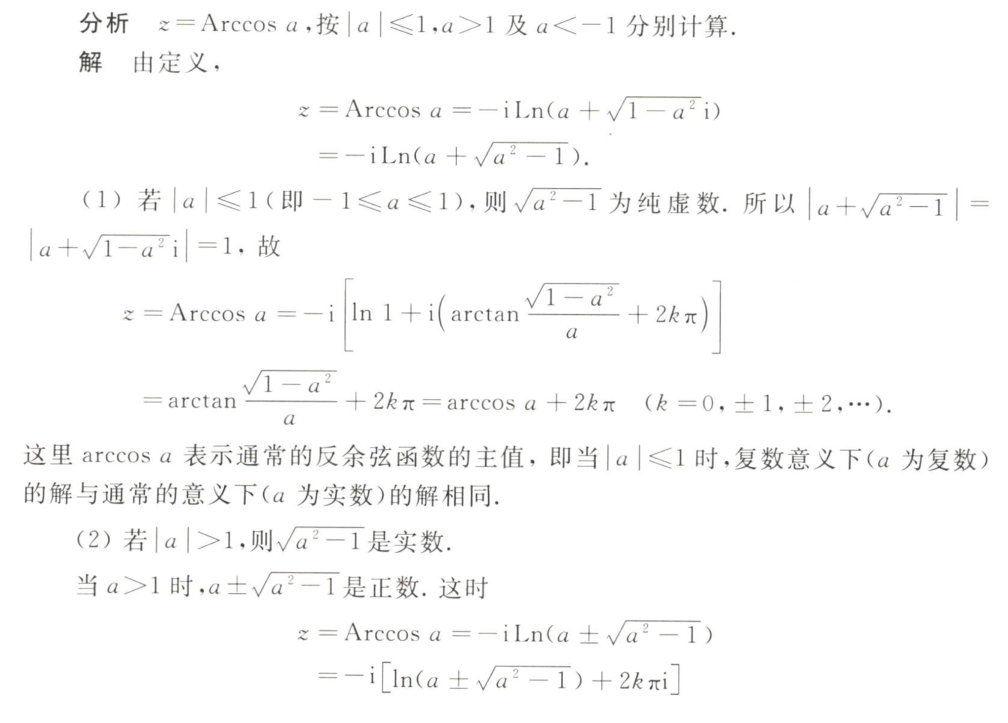
\includegraphics[width=\textwidth]{38-解析函数-20250320.png}
% \caption{}
\label{}
\end{figure}

\begin{figure}[H]
\centering
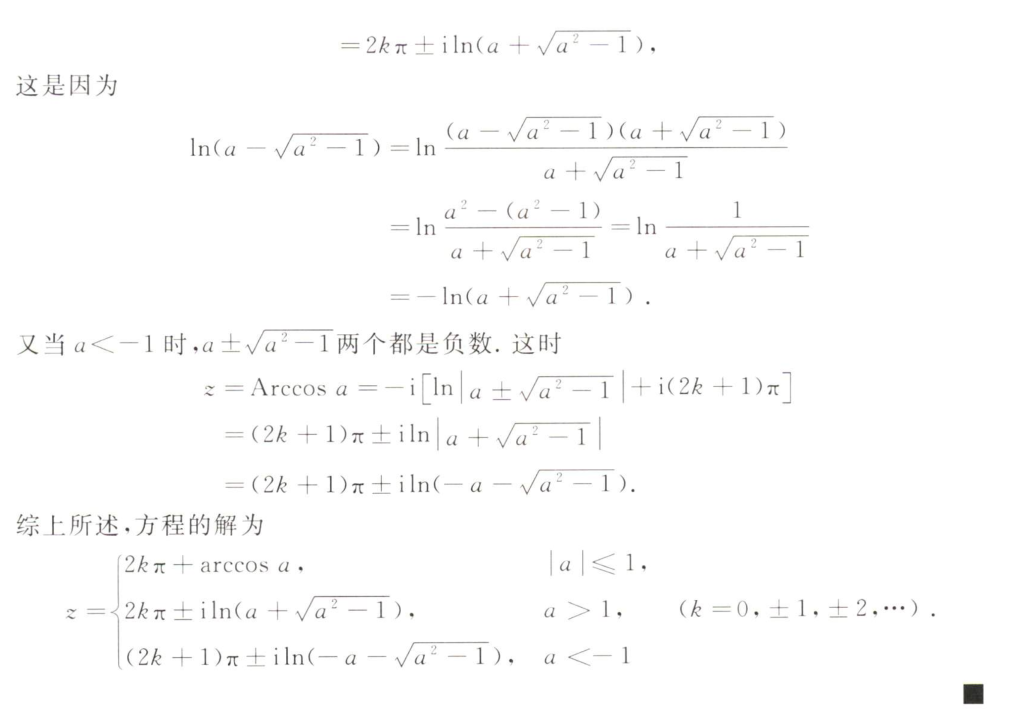
\includegraphics[width=\textwidth]{39-解析函数-20250320.png}
% \caption{}
\label{}
\end{figure}

\begin{exercise}
\begin{figure}[H]
\centering
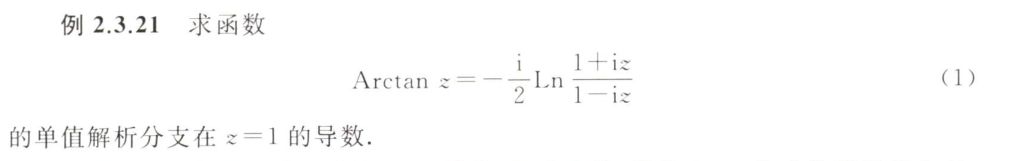
\includegraphics[width=\textwidth]{40-解析函数-20250320.png}
% \caption{}
\label{}
\end{figure}
\end{exercise}
\begin{note}
变量代换 $\zeta=\frac{1+iz}{1-iz}$,化简,并将 $\mathrm{Ln}\  z$ 分成单值解析分支,然后就可以按照复合函数求导。
\end{note}
\begin{figure}[H]
\centering
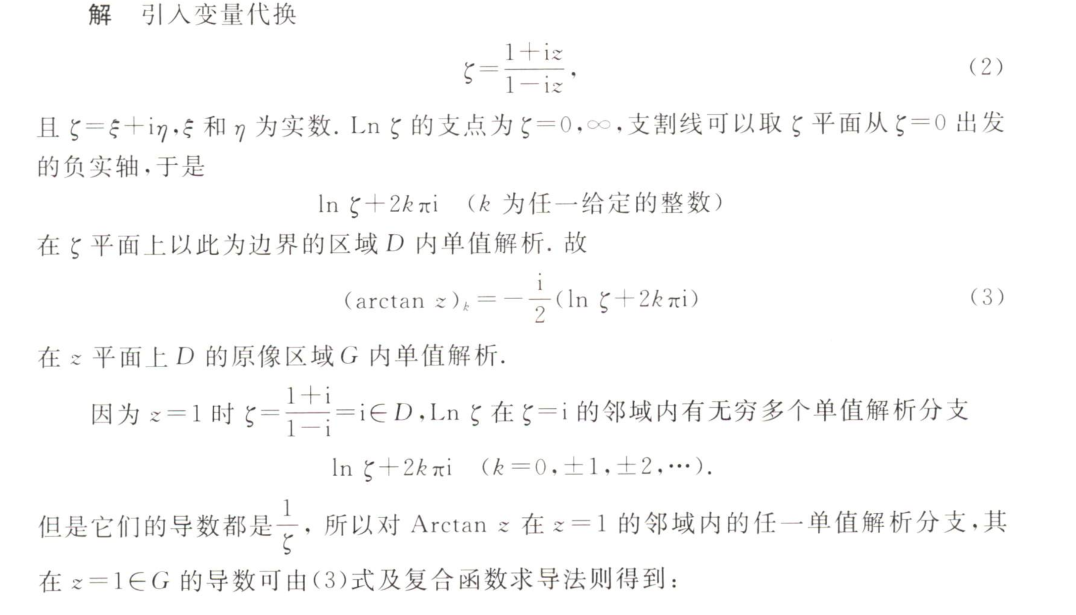
\includegraphics[width=\textwidth]{41-解析函数-20250320.png}
% \caption{}
\label{}
\end{figure}

\begin{figure}[H]
\centering
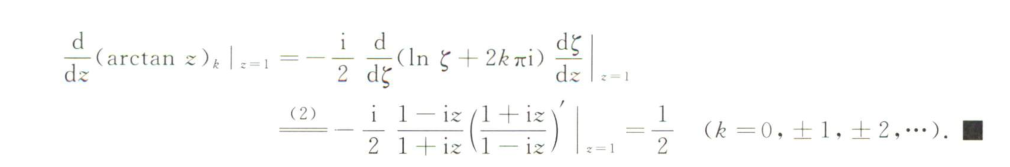
\includegraphics[width=\textwidth]{42-解析函数-20250320.png}
% \caption{}
\label{}
\end{figure}
